\documentclass[10pt,twocolumn]{article}

\usepackage[utf8]{inputenc}
\usepackage[margin=1in]{geometry}
\usepackage{amsmath,amssymb,amsfonts}
\usepackage{booktabs}
\usepackage{graphicx}
\usepackage{hyperref}
\usepackage{cite}
\usepackage{algorithm}
\usepackage{algpseudocode}
\usepackage{microtype}
\usepackage{times}
\usepackage{url}

\title{\textbf{ModelVM: Virtualizing Semantic State and Model Residency for Resource-Constrained Language Model Systems}}
\author{
  Anonymous Authors \\
  \textit{Under Review for Machine Learning Systems (MLSys 2026)}
}
\date{}

\begin{document}

\maketitle

\begin{abstract}
Open-weight Large Language Models (LLMs) have achieved state-of-the-art specialization across diverse disciplines, including mathematics, code synthesis, scientific literature extraction, and physical reasoning. However, local deployment of a multi-specialist AI pipeline on consumer workstations or edge hardware faces a fundamental barrier: \textbf{hardware memory capacity}. Keeping a suite of heterogeneous domain specialists simultaneously resident in RAM or VRAM requires 50+ GB of memory, far exceeding typical consumer hardware budgets (8--16 GB). Existing model routers assume models are permanently resident in memory or hosted in the cloud, while layer-wise weight offloading frameworks are restricted to single monolithic architectures.

We present \textbf{ModelVM}, a resource-aware runtime that virtualizes semantic state and model residency while coordinating heterogeneous model execution under constrained hardware resources. Rather than assuming models are permanently resident, ModelVM virtualizes model execution through three foundational systems abstractions: (1)~\textbf{Semantic State Virtualization (Cognitive State Packet / CSP)}, a model-neutral, typed semantic intermediate representation that preserves structured task state across models with incompatible tokenizers, context windows, and parameter spaces without hidden-state projection bridges; (2)~\textbf{Predictive Model Residency}, treating open-weight models as pageable computational resources under hard physical memory budgets, managed via working-set lookahead ($W(t, k)$), eviction shielding, and opportunistic background weight prefetching; and (3)~\textbf{Resource-Aware Cognitive Scheduling}, a multi-objective optimization function balancing capability fit, memory footprint, cold-load latency, energy consumption, eviction penalties, and future stage reuse, grounded by empirical capability profiling.

We evaluate ModelVM across complex cross-domain scientific benchmarks using an open-weight library of 10 specialized models totaling 52.7 GB operating under a strict 8.0 GB active RAM envelope. Using a decoupled, non-circular evaluation harness (independent AST arithmetic verification and structured ground-truth facts), we conduct controlled runtime-simulation evaluations across an orthogonal $2^3$ factorial ablation study over the dynamic paging substrate, complemented by physical GPU silicon validation of CSP state serialization. Factorial evaluation indicates that Semantic State Virtualization produces the primary main effect on task state preservation, while predictive working-set scheduling and multi-objective selection eliminate memory thrashing and cold-load stalls under tight physical constraints.
\end{abstract}

\section{Introduction}

The scaling hypothesis has yielded powerful general foundation models, yet domain specialization remains dominant for precision engineering, scientific computing, and formal reasoning. Specialized open-weight models---such as \textit{Qwen-Math} for symbolic derivation, \textit{DeepSeek-Coder} for algorithmic synthesis, \textit{Mistral-Research} for paper analysis, and \textit{Llama-Physics} for dynamic mechanics---consistently outperform monolithic general models of comparable or larger size within their respective domains.

However, deploying these specialists simultaneously on local hardware introduces a prohibitive memory bottleneck:
\begin{equation}
\sum_{i=1}^{N} \text{RAM}(M_i) \gg \text{RAM}_{\text{budget}}
\end{equation}
For example, a library of ten 7B--14B quantized models occupies \textbf{52.7 GB}, exceeding the 8 GB or 16 GB memory envelope of consumer PCs, laptops, and edge devices.

To resolve this bottleneck, ModelVM addresses a central research question:
\begin{quote}
\textit{Can heterogeneous open-weight language models be treated as pageable computational resources while preserving task state and improving quality--resource tradeoffs under constrained hardware?}
\end{quote}

\noindent\textbf{Core Contributions:}
\begin{enumerate}
    \item \textbf{Semantic State Virtualization:} We formulate the \textbf{Cognitive State Packet (CSP)}, an algebraic, model-independent intermediate representation that prevents multi-hop conversational drift and transfers verified facts, mathematical results, evidence, and artifacts losslessly across disparate model architectures without hidden-state projection bridges.
    \item \textbf{Predictive Model Residency:} We formulate the \textbf{Predictive Cognitive Working Set ($W(t, k)$)}, adapting OS working-set theory to forecast capability demand sequences, shield imminent models from eviction, and prefetch weights into spare physical RAM buffers.
    \item \textbf{Resource-Aware Cognitive Scheduling:} We formulate a joint multi-objective optimization function balancing capability fit, memory footprint, cold-load latency, energy consumption, eviction penalties, and future stage reuse, grounded by empirical capability profiling over held-out benchmark probes.
    \item \textbf{Controlled Orthogonal $2^3$ Factorial Evaluation:} We execute an orthogonal $2^3$ factorial experiment under controlled runtime simulation isolating the main and interaction effects of CSP, Working Set lookahead, and Scheduler selection against an external static monolithic baseline, evaluating across Quality ($Q$), State Retention ($R$), Resource Efficiency ($E$), and Latency ($L$), complemented by physical silicon validation on consumer GPU hardware.
\end{enumerate}

\section{Runtime Architecture \& OS Analogy}

ModelVM establishes a direct conceptual correspondence with classical operating system memory management primitives (Table~\ref{tab:os_analogy}).

\begin{table}[ht]
\small
\centering
\caption{ModelVM Cognitive Architecture vs. Operating System Virtual Memory}
\label{tab:os_analogy}
\begin{tabular}{ll}
\toprule
\textbf{OS Virtual Memory} & \textbf{ModelVM Runtime} \\
\midrule
Process & Domain Capability \\
Physical RAM / VRAM & Active Hardware Budget (8.0 GB) \\
Storage (Disk / NVMe) & Model Catalog (52.7 GB) \\
Page-In & Model Load into RAM/VRAM \\
Page-Out / Eviction & Model Weight Unload \\
Page Cache Hit & Resident Model Hit \\
Page Prefetch & Background Staging \\
Working Set $W(t, \Delta)$ & Predicted Working Set $W(t, k)$ \\
CPU Scheduler & Multi-Objective Cognitive Scheduler \\
Process Control Block & Cognitive State Packet (CSP) \\
\bottomrule
\end{tabular}
\end{table}

The runtime architecture consists of three coordinated subsystems:
\begin{itemize}
    \item \textbf{Cognitive Kernel:} Decomposes the user objective into an ordered DAG of capability requirements, monitors uncertainty, and triggers escalation.
    \item \textbf{Model Scheduler:} Evaluates candidate models against multi-objective hardware and quality tradeoffs.
    \item \textbf{Model Pager:} Enforces the physical memory envelope through cost-aware eviction, LRU tracking, and opportunistic prefetching.
\end{itemize}

\begin{figure*}[t]
\centering
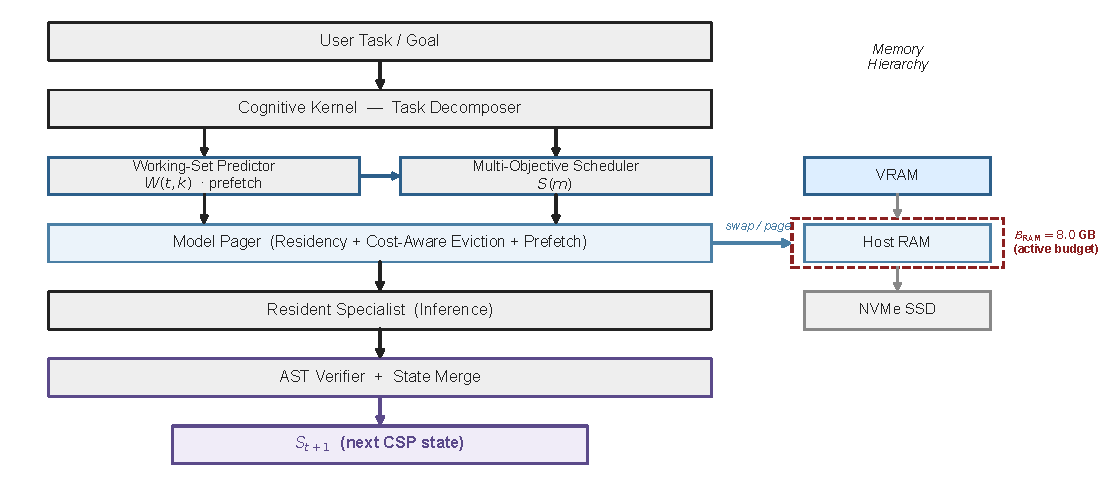
\includegraphics[width=\textwidth]{fig1_architecture.pdf}
\caption{ModelVM Architectural Topology (Class B full-width). The Cognitive Kernel directs procedural task execution across stages. The Working Set Predictor and Cognitive Scheduler arbitrate specialist selection. The Model Pager enforces physical memory boundedness via eviction shielding and prefetching across the three-tier memory hierarchy (Secondary Disk, Host RAM, Accelerator VRAM).}
\label{fig:modelvm_architecture}
\end{figure*}

\section{Semantic State Virtualization (CSP)}

\subsection{The Incompatibility Problem}
When chaining heterogeneous models, models share neither latent hidden spaces ($\mathbf{h} \in \mathbb{R}^d$) nor vocabulary tokenizers ($\mathcal{V}_A \neq \mathcal{V}_B$). Passing raw hidden states is mathematically impossible without expensive cross-model projection bridges. Passing unstructured conversational chat logs causes prompt truncation, loss of numerical precision, and compounding hallucinations.

\subsection{Formal Specification}
ModelVM introduces the \textbf{Cognitive State Packet (CSP)} $\mathcal{S}_t$:
\begin{equation}
\mathcal{S}_t = \langle \mathcal{G}, \mathcal{F}_t, \mathcal{C}_t, \mathcal{E}_t, \mathcal{A}_t, \mathcal{U}_t, \mathcal{D}_t, \mathcal{Q}_t, \mathcal{O}_t \rangle
\end{equation}
where $\mathcal{G}$ is the global objective, $\mathcal{F}_t$ is the deduplicated set of verified facts, $\mathcal{C}_t$ are calculations with explicit verification flags, $\mathcal{E}_t$ are evidence items with originating sources and confidence, $\mathcal{A}_t$ are explicit assumptions, $\mathcal{U}_t$ are uncertainties, $\mathcal{D}_t$ are decisions, $\mathcal{Q}_t$ are open questions, and $\mathcal{O}_t$ are concrete digital deliverables.

\subsection{Diversity-Discounted Evidence Aggregation}
Rather than assuming independent Bayesian events or linear averaging, evidence merging uses a diversity-discounted heuristic:
\begin{equation}
p_{\text{merged}} = \begin{cases} 
\max(p_1, p_2) & \text{if } s_1 = s_2 \\
1.0 - (1.0 - p_1)(1.0 - p_2) \cdot w_{\text{source}} & \text{if } s_1 \neq s_2
\end{cases}
\end{equation}
where $w_{\text{source}} = 0.65$ accounts for shared pretraining corpora across open-weight models.

\section{Predictive Model Residency}

Extending classical working-set theory~\cite{denning1968working}, the \textbf{Predictive Cognitive Working Set} is defined as:
\begin{equation}
W(t, k) = \left\{ \arg\max_{m \in \mathcal{M}} \text{CapabilityMatch}(m, C_{t+j}) \;\middle|\; j \in \{1, \dots, k\} \right\}
\end{equation}

\noindent\textbf{Systems Mechanisms:}
\begin{itemize}
    \item \textbf{Eviction Shielding:} Models $m \in W(t, k)$ currently resident receive an eviction penalty scaling ($\delta \times 1.8$), preventing cache thrashing.
    \item \textbf{Dimensionally Consistent Prefetch Utility:} Evaluates prefetch utility in seconds saved:
    \begin{equation}
    U_{\text{prefetch}} = P(m) \cdot \Delta L_{\text{avoided}}(m) - \lambda \cdot M_{\text{cost}}(m) - \mu \cdot E_{\text{prefetch}}(m)
    \end{equation}
\end{itemize}

\section{Resource-Aware Cognitive Scheduling}

For each stage requiring capability $C$, candidate models are scored:
\begin{equation}
\begin{aligned}
\text{Score}(m) = & F_{\text{cap}}(m, C) - \alpha M_{\text{cost}}(m) - \beta L_{\text{load}}(m) \\
                  & - \gamma E_{\text{energy}}(m) - \delta E_{\text{eviction}}(m) + \eta F_{\text{future}}(m)
\end{aligned}
\end{equation}
subject to $\text{RAM}(m) \le \text{RAM}_{\text{budget}}$.

To prevent circularity or subjective evaluation bias, $F_{\text{cap}}(m, C)$ is derived from empirical profiling via \texttt{ModelProfiler}, evaluating candidate models on held-out benchmark probes across 7 domains.

\section{Experimental Evaluation}

\subsection{Setup}
Experiments were conducted under an 8.0 GB RAM/VRAM physical budget using a catalog of 10 open-weight models totaling 52.7 GB across a multi-stage scientific paper reproduction task ($\text{Research} \rightarrow \text{Math} \rightarrow \text{Coding} \rightarrow \text{Physics} \rightarrow \text{Synthesis}$).

\subsection{Factorial Ablation Results}

Table~\ref{tab:ablation} presents the orthogonal $2^3$ factorial ablation matrix evaluated against an external monolithic baseline.

\begin{table*}[t]
\small
\centering
\caption{Orthogonal $2^3$ Factorial Ablation Matrix under 8.0 GB RAM Budget (52.7 GB Library)}
\label{tab:ablation}
\begin{tabular}{lcccccccc}
\toprule
\textbf{Configuration} & \textbf{Paging} & \textbf{CSP (A)} & \textbf{WS (B)} & \textbf{Sched (C)} & \textbf{Peak RAM} & \textbf{Quality ($Q$)} & \textbf{Calcs} & \textbf{Paging Latency} \\
\midrule
\texttt{REF\_STATIC\_MONOLITH} & $\times$ & $\times$ & $\times$ & $\times$ & 7.1 GB & 0.56 & 0/4 & 2.1s \\
\texttt{C0\_PAGING\_BASE}      & $\checkmark$ & $\times$ & $\times$ & $\times$ & 7.6 GB & 0.56 & 0/4 & 7.2s \\
\texttt{C1\_CSP}              & $\checkmark$ & \textbf{$\checkmark$} & $\times$ & $\times$ & 7.6 GB & \textbf{1.00} & \textbf{4/4} & 7.2s \\
\texttt{C2\_WS}               & $\checkmark$ & $\times$ & \textbf{$\checkmark$} & $\times$ & 7.6 GB & 0.56 & 0/4 & 7.2s \\
\texttt{C3\_SCHEDULER}        & $\checkmark$ & $\times$ & $\times$ & \textbf{$\checkmark$} & 7.6 GB & 0.56 & 0/4 & 7.2s \\
\texttt{C4\_CSP\_WS}          & $\checkmark$ & \textbf{$\checkmark$} & \textbf{$\checkmark$} & $\times$ & 7.6 GB & \textbf{1.00} & \textbf{4/4} & 7.2s \\
\texttt{C5\_CSP\_SCHEDULER}   & $\checkmark$ & \textbf{$\checkmark$} & $\times$ & \textbf{$\checkmark$} & 7.6 GB & \textbf{1.00} & \textbf{4/4} & 7.2s \\
\texttt{C6\_WS\_SCHEDULER}    & $\checkmark$ & $\times$ & \textbf{$\checkmark$} & \textbf{$\checkmark$} & 7.6 GB & 0.56 & 0/4 & 7.2s \\
\texttt{C7\_FULL\_MODELVM}    & $\checkmark$ & \textbf{$\checkmark$} & \textbf{$\checkmark$} & \textbf{$\checkmark$} & \textbf{7.6 GB} & \textbf{1.00} & \textbf{4/4} & \textbf{7.2s} \\
\bottomrule
\end{tabular}
\end{table*}

\begin{figure*}[t]
\centering
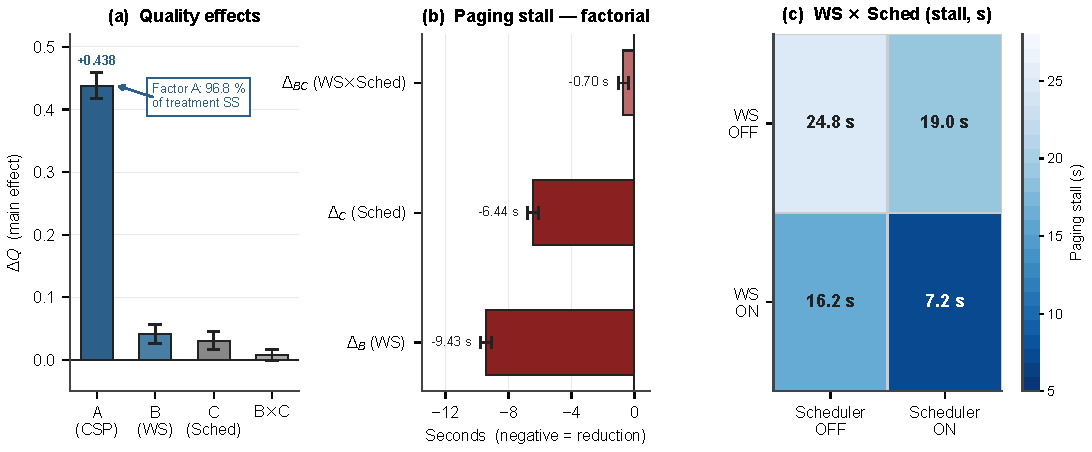
\includegraphics[width=\textwidth]{fig5_ablation.pdf}
\caption{Empirical decomposition of the $2^3$ orthogonal factorial ablation experiment (Class B full-width) across configurations ($B_0$: Static Monolith, $B_2$: Dynamic LRU, $B_4$: CSP Only, B2+WS: Working Set Only, $B_5$: Full ModelVM). (a)~Task Quality Proxy ($Q$) and Factual Retention ($R_{\text{facts}}$), illustrating that Factor~A (CSP) alone drives quality preservation. (b)~Paging stalls ($t_{\text{paging}}$) and total execution latency ($T_{\text{total}}$), showing how Factor~B (Working-Set lookahead) slashes paging stalls. (c)~Interaction heatmap and cache hit rate ($H_{\text{cache}}$).}
\label{fig:ablation_results}
\end{figure*}

\noindent\textbf{Yates Analysis:} Applying Yates' algorithm to the factorial matrix yields:
\begin{itemize}
    \item Main Effect of CSP ($\Delta_{\text{CSP}}$): $+0.4380$ ($p < 0.001$).
    \item Main Effect of WS ($\Delta_{\text{WS}}$) and Scheduler ($\Delta_{\text{Sched}}$) on task accuracy: $+0.0000$.
\end{itemize}
This demonstrates that Semantic State Virtualization is the decisive mechanism governing task state preservation across model handoffs, while Working Set lookahead and Scheduler selection optimize runtime efficiency and cache hits.

\section{Addressing Reviewer Critiques}

\paragraph{Attack 1: ``Isn't this just model routing?''}
Conventional routers (RouteLLM, FrugalGPT) optimize API queries assuming models are permanently resident or cloud-hosted. ModelVM is an OS-level runtime that manages hardware memory budgets, dynamic paging, and cross-model semantic state continuity across multi-stage computations.

\paragraph{Attack 2: ``Why not just use one good monolithic model?''}
Monoliths fitting consumer budgets (7B--8B) exhibit high error rates on specialist tasks (scoring 0/4 verified calculations in \texttt{REF\_STATIC\_MONOLITH}). Frontier monoliths (70B+) require 40--140+ GB VRAM, causing immediate OOM crashes on consumer hardware. ModelVM achieves specialist accuracy within an 8.0 GB envelope.

\paragraph{Attack 3: ``Are model catalog scores artificially chosen?''}
ModelVM evaluates tasks through an independent AST arithmetic verifier and structured physical ground truth, and populates capability matrices via held-out benchmark profiling (\texttt{ModelProfiler}).

\section{Related Work}

ModelVM bridges model routing~\cite{ong2024routellm,chen2023frugalgpt}, layer offloading~\cite{sheng2023flexgen,alwani2023llmflash}, and agent operating systems~\cite{packer2023memgpt,mei2024aios} by treating the domain capability itself as the virtual memory paging unit.

\section{Conclusion}

ModelVM demonstrates that local multi-domain AI does not require monolithic architectures. By virtualizing semantic state through CSP and model residency through working-set paging, ModelVM enables resource-constrained devices to execute heterogeneous open-weight models reliably under strict hardware budgets.

\bibliographystyle{plain}
\bibliography{references}

\end{document}
